\subsection{Semaforo privo di enable}
Si vuole innanzitutto realizzare una FSM che alterni gli stati come descritto nella sezione precedente.
Avendo tre stati diversi è necessario impiegare almeno 2 flip-flop; non abbiamo avuto necessità di utilizzarne ulteriori: si riporta la codifica scelta in
\tab{cod} e lo schema di stati e transizioni in \fig{stati}, dove LV, LG e LR indicano LED Verde, Giallo e Rosso rispettivamente. Una tale codifica impone $b_{0}^{n+1} =  \overline{b_{1}^{n} \cdot b_{0}^{n}}$ e $b_{1}^{n+1} = b_{0}^{n}$; in tal modo lo stato indesiderato $00$, non corrispondente a nessuno degli stati codificati, ha comunque una transizione accettabile senza richiedere logica ulteriore.

Si riporta la \tablename{ \ref{tab:tran}} delle transizioni tra i vari stati della FSM, assieme allo stato desiderato degli output della macchina; tali output sono ottenibili come:
$$LV = b_1 \qquad LG = \overline{b_0} \qquad LR = \overline{b_1}$$

Tali segnali sono ricavabili direttamente agli output $Q$ e $\qbar$ dei D-Latch utilizzati, senza logica aggiuntiva; la FSM progettata è dunque di Moore, dal momento che l'output dipende solo dallo stato.

Per realizzare la FSM basata sugli integrati a disposizione, e che realizzi quanto appena descritto,
è stato dunque realizzato il circuito in \figurename{ \ref{fig:sem2}} alimentando la componentistica con una tensione
$V_{cc}\approx \SI{5}{\volt}$. In serie con i LED sono state montate delle resistenze $R\approx 330$ \si{\ohm} per limitare la richiesta di corrente dei LED stessi.

\begin{figure}[h!]
\begin{minipage}{0.5\textwidth}
		\centering
		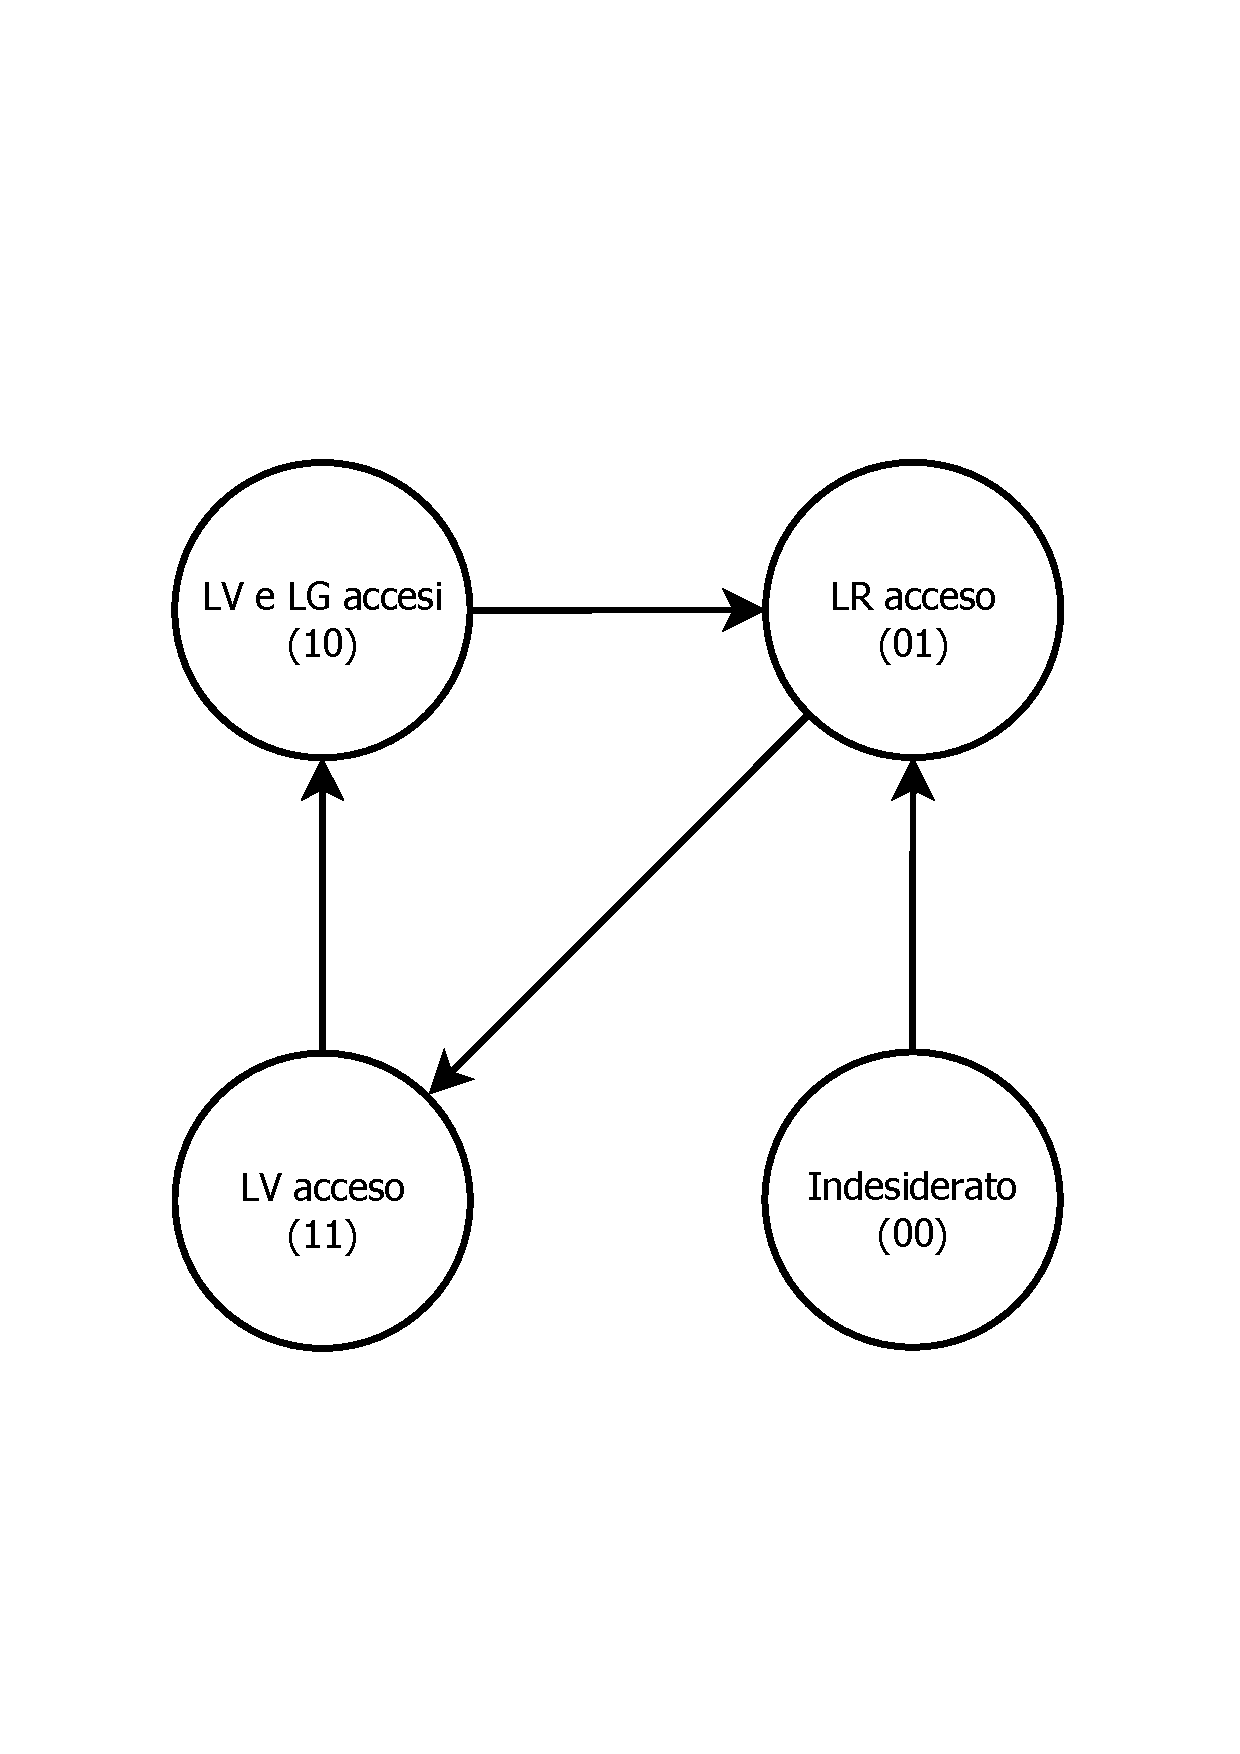
\includegraphics[scale=0.4,trim={0 6cm 0 6cm},clip]{stati_no_enable.pdf}
		\caption{Stati della FSM semaforo senza En.}
		\label{fig:stati}
\end{minipage}
\begin{minipage}{0.5\textwidth}
		\centering
		\begin{tabular}{ssc}
		\toprule
		b_1 & b_0 & stato corrispondente\\
		\midrule
		1 & 1 & VERDE\\
		1 & 0 & GIALLO \& VERDE\\
		0 & 1 & ROSSO\\
		0 & 0 &  X (NON VOLUTO)\\
		\bottomrule
		\end{tabular}
		\captionof{table}{Codifica degli stati impiegati}
		\label{tab:cod}
\end{minipage}
\end{figure}

\begin{table}[h]
\centering
\begin{tabular}{cc|cc|ccc}
	\toprule
	b_{1}^{n} & b_{0}^{n}  & b_{1}^{n+1} & b_{0}^{n+1} & \text{LED VERDE} & \text{LED GIALLO} & \text{LED ROSSO} \\
	\midrule
	 0 & 0 & 0 & 1  & x (0) & x (1) & x (1) \\
	 0 & 1 & 1 & 1  & 0 & 0 & 1  \\
	 1 & 1 & 1 & 0  & 1 & 0 & 0 \\
	 1 & 0 & 0 & 1  & 1 & 1 & 0 \\
	\bottomrule
\end{tabular}
\caption{Tabella delle transizioni della FSM semaforo sempre abilitato; tra parentesi gli output effettivi del nostro circuito per stati indesiderati.}
\label{tab:tran}
\end{table}

\begin{figure}[h!]
	\centering
	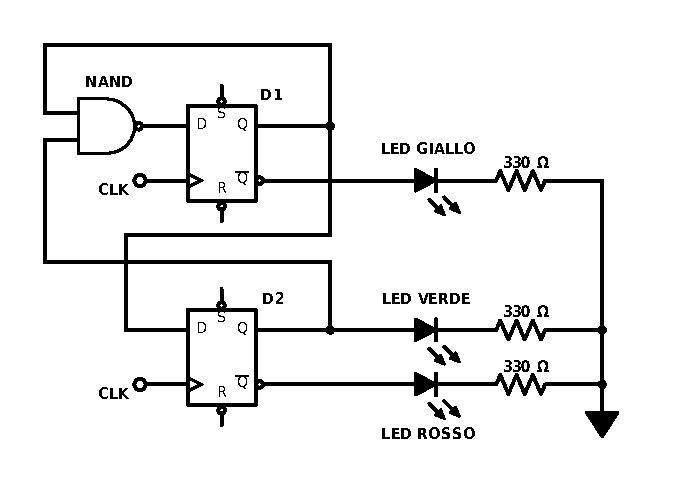
\includegraphics[scale=1.0]{no_enable.pdf}
	\caption{Circuito che realizzi il semaforo senza En.}
	\label{fig:sem2}
\end{figure}

Per la verifica del funzionamento circuitale è stato
inviato un segnale di clock di frequenza bassa ($\sim \SI{1}{\Hz}$) e effettuando un primo controllo attraverso l'accensione dei LED. Si è successivamente aumentata la frequenza di clock a $f= \SI{175.937\pm 0.001}{\hertz}$\footnote{Tale misura è stata presa con la funzione di acqusizione automatica dell'oscilloscopio; l'incertezza associata è la prima cifra che risulti stabile.}
ed acquisito i valori di tensione corrispondente alle uscite dei vari LED, riportate in
\figurename{ \ref{fig:acq}}. Dall'osservazione di
tali acquisizioni si verifica l'accordo con le specifiche attese.

\begin{figure}[h]
	\centering
	\subfloat[clock ch.1  LED VERDE ch. 2]{
		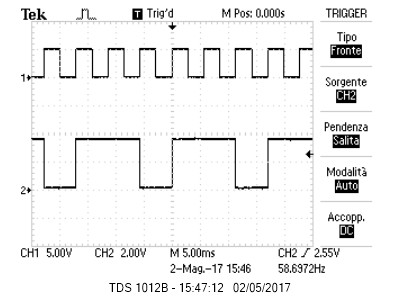
\includegraphics[scale=0.3]{semaforosemplice/verde.bmp}
	}
	\subfloat[clock ch.1 LED GIALLO ch.2]{
		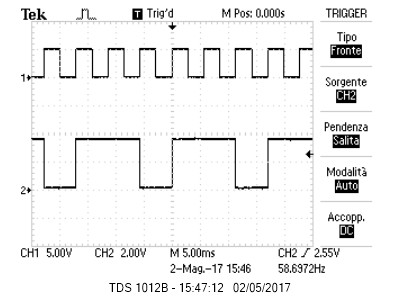
\includegraphics[scale=0.3]{semaforosemplice/giallo.bmp}
		}\\
	\subfloat[clock ch.1  LED ROSSO ch.2]{
		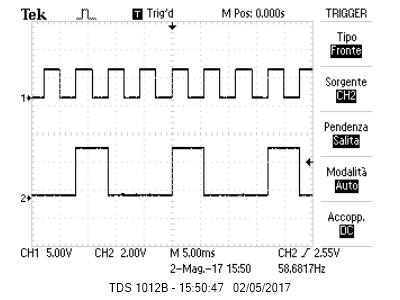
\includegraphics[scale=0.3]{semaforosemplice/rosso.bmp}
		}
	\subfloat[clock ch.1  $b_{0}$ ch.2]{
		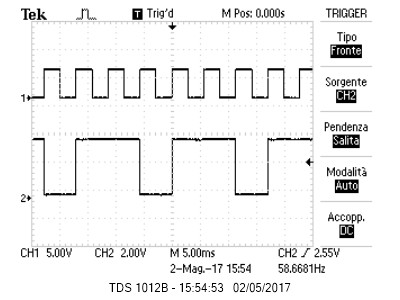
\includegraphics[scale=0.3]{semaforosemplice/q-.bmp}
		}\\
	\subfloat[clock ch.1 $b_{1}$  ch.2]{
		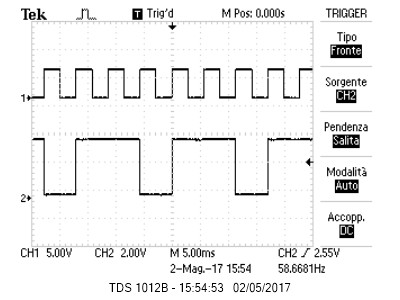
\includegraphics[scale=0.3]{semaforosemplice/q+.bmp}
	}

	\subfloat[verde ch.1, giallo  ch.2]{
		\includegraphics[scale=0.3]{semaforosemplice/verde giallo.bmp}
	}
	\subfloat[verde ch.1, rosso  ch.2]{
		\includegraphics[scale=0.3]{semaforosemplice/verde rossoo.bmp}
	}
\caption{Acquisizione telle tensioni osservate nel semaforo privo di ENABLE}
\label{fig:acq}
\end{figure}
